\documentclass[a4paper,12pt]{article}
\usepackage[top = 2.5cm, bottom = 2.5cm, left = 2.5cm, right = 2.5cm]{geometry} 
\usepackage[T1]{fontenc}
\usepackage[utf8]{inputenc}
\usepackage{multirow}
\usepackage{booktabs}
\usepackage{graphicx} 
\usepackage{setspace}
\setlength{\parindent}{0in}
\usepackage{float}
\usepackage{fancyhdr}
\usepackage[table,xcdraw]{xcolor}
\pagestyle{fancy}
\fancyhf{}
\lhead{\footnotesize GEO1001: Homework 1}
\rhead{\footnotesize Georgios Triantafyllou (5381738)}
\cfoot{\footnotesize \thepage} 

\begin{document}
	\thispagestyle{empty}
	\begin{tabular}{p{15.5cm}}
		{\large \bf Sensing Technologies and Mathematics for Geomatics} \\
		GEO1001.2020 \\ MSc Geomatics \\ Delft University of Technology \\
		\hline
	\end{tabular} 
\vspace*{0.3cm}
\begin{center}
	{\Large \bf Homework 1}
	\vspace{2mm}
	{\bf Georgios Triantafyllou (5381738)}
\end{center} 
\vspace{0.4cm}
\section{A1}
 \subsection{A1.1}
From the results i have, there are no many things that could be said. It would be adviseble and needed further analysis in order to reach some conclusion because the amount of data for each sensor are really big.
 \subsection{A1.2}
The number of bins it is really important because if we use too few of them, the histogram does not really portray the data very well (Figure 1). From the other side if we have too many bins, we get a broken comb look, which also does not give a good sense of the distribution (Figure 2). A good example is visible in to the next histograms.
  \begin{figure}[H] 
	\centering
	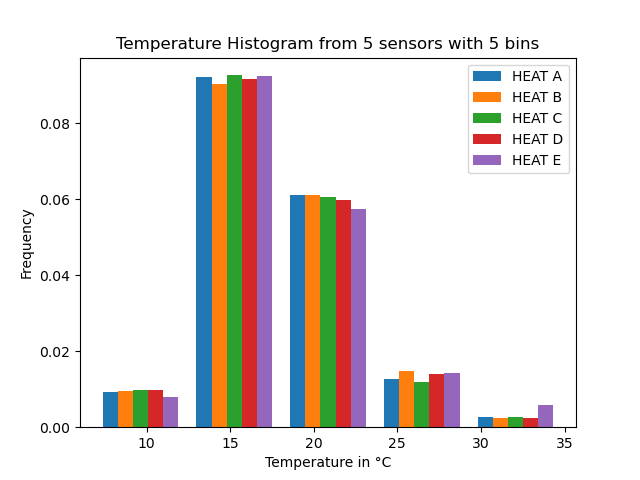
\includegraphics[width=0.7\textwidth]{Temperature Histogram from 5 sensors with 5 bins.png}
	\caption{Temperature Histogram from 5 sensors with 5 bins\cite{Maiullari2020}}
  \end{figure}
  \begin{figure}[H] 
	\centering
	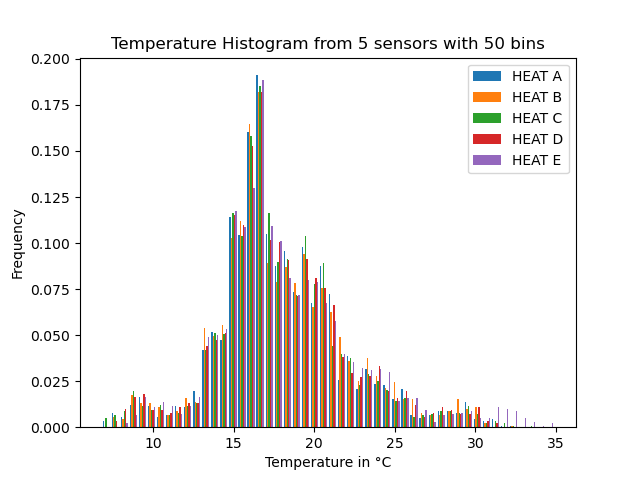
\includegraphics[width=0.7\textwidth]{Temperature Histogram from 5 sensors with 50 bins.png}
	\caption{Temperature Histogram from 5 sensors with 50 bins\cite{Maiullari2020}}
  \end{figure}

 \subsection{A1.3}
  \begin{figure}[H] 
	\centering
	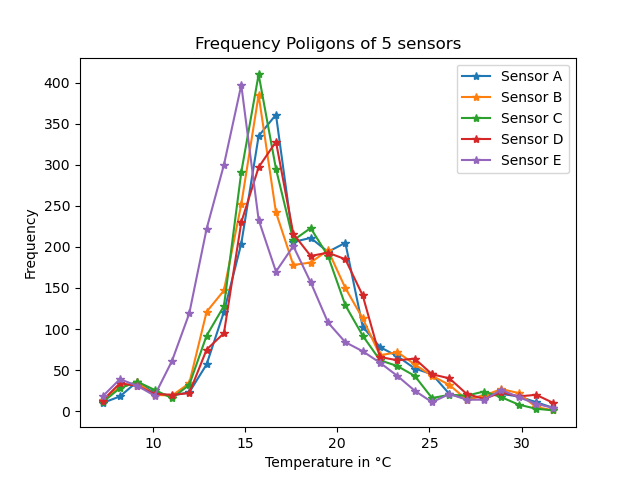
\includegraphics[width=0.7\textwidth]{Frequency Poligons of 5 Sensors.png}
	\caption{Frequency Poligons of 5 Sensors\cite{Maiullari2020}}
  \end{figure}

 \subsection{A1.4}
  \begin{figure}[H] 
	\centering
	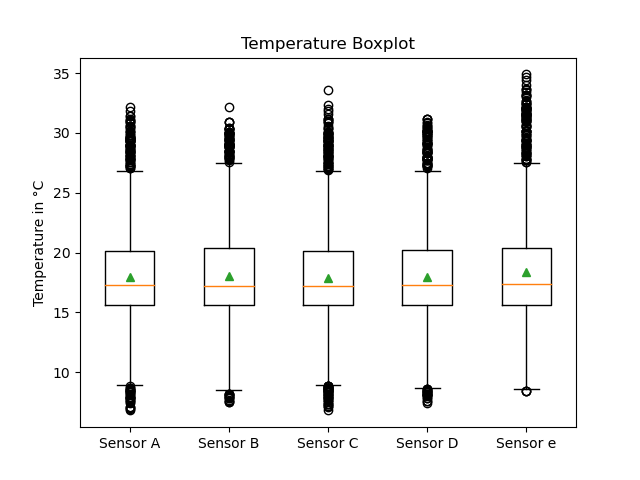
\includegraphics[width=0.7\textwidth]{Temperature Boxplot.png}
	\caption{Temperature Boxplot\cite{Maiullari2020}}
  \end{figure}
  \begin{figure}[H] 
	\centering
	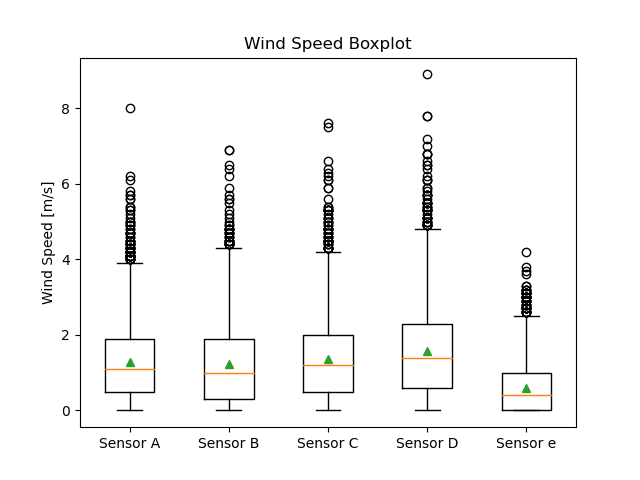
\includegraphics[width=0.7\textwidth]{Wind Speed Boxplot.png}
	\caption{Wind Speed Boxplot\cite{Maiullari2020}}
  \end{figure}
  \begin{figure}[H] 
	\centering
	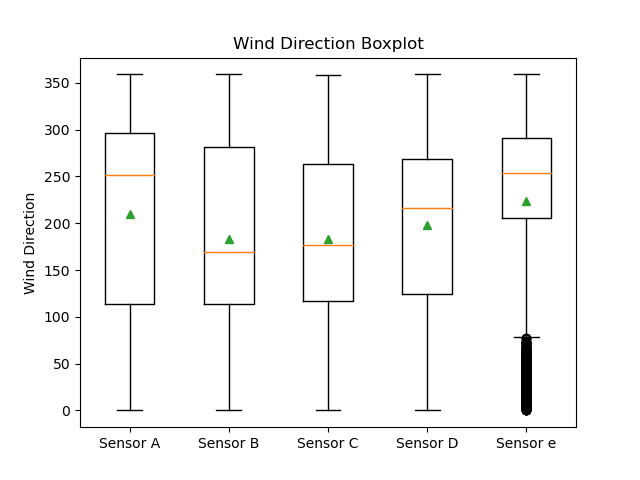
\includegraphics[width=0.7\textwidth]{Wind Direction Boxplot.png}
	\caption{Wind Direction Boxplot\cite{Maiullari2020}}
  \end{figure}
\pagebreak
\section{A2}
 \subsection{A2.1}
 From the figures below we can realize that the behavior of the distributions for each Sensor's Temperature look pretty similar when we look the PDF and PMF (Figures 7,8) while the CDF is totally diferent because it is comulative distribution (Figure 9). As about their tails i could talk only for PMF and PDF where it could be said that in PDF the tail is longer somehow and thats because its more smooth than in PMF. More can be seen in the Figures below:
 \samepage
  \begin{figure}[H] 
	\centering
	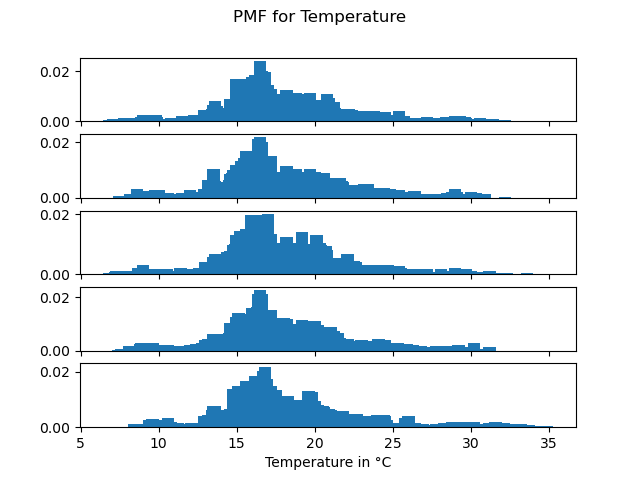
\includegraphics[width=0.7\textwidth]{PMF for Temperature.png}
	\caption{PMF for Temperature\cite{Maiullari2020}}
  \end{figure}
  \begin{figure}[H] 
	\centering
	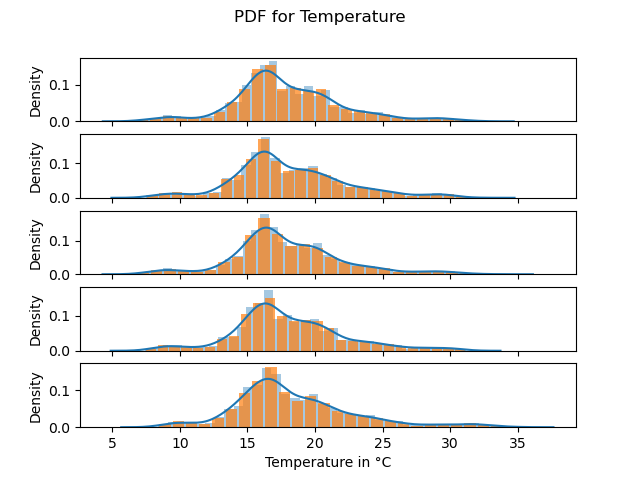
\includegraphics[width=0.7\textwidth]{PDF for Temperature.png}
	\caption{PDF for Temperature\cite{Maiullari2020}}
  \end{figure}
  \begin{figure}[H] 
	\centering
	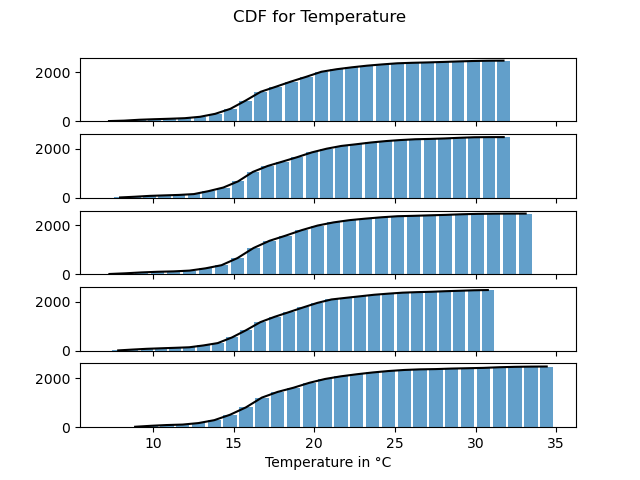
\includegraphics[width=0.7\textwidth]{CDF for Temperature.png}
	\caption{CDF for Temperature\cite{Maiullari2020}}
  \end{figure}
\pagebreak
 \subsection{A2.2}
 From the figures below we can see that there is no actual diference between the PDF and the Kernel Density Estimation (KDE) for the Wind Speed and that happens because the KDE is actually an algorithm that takes a sample
 and finds an appropriately smooth PDF that fits the data. So the only diference is that the KDE shows less information in the graph and makes it easier for the audience to understand it.
  \begin{figure}[H] 
	\centering
	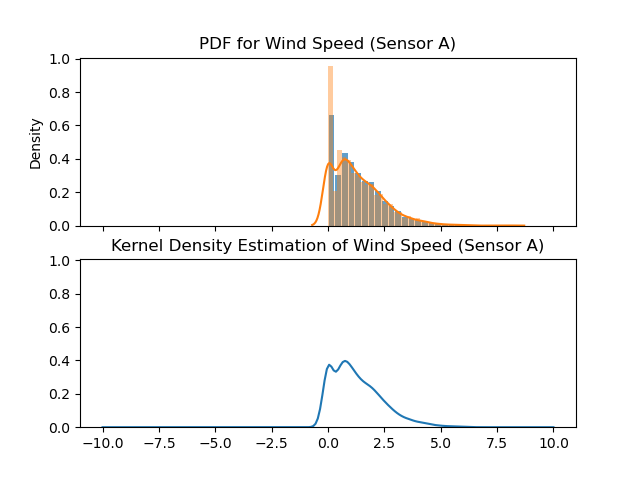
\includegraphics[width=0.7\textwidth]{PDF for Wind Speed (Sensor A).png}
	\caption{PDF for Wind Speed (Sensor A)\cite{Maiullari2020}}
  \end{figure}
  \begin{figure}[H] 
	\centering
	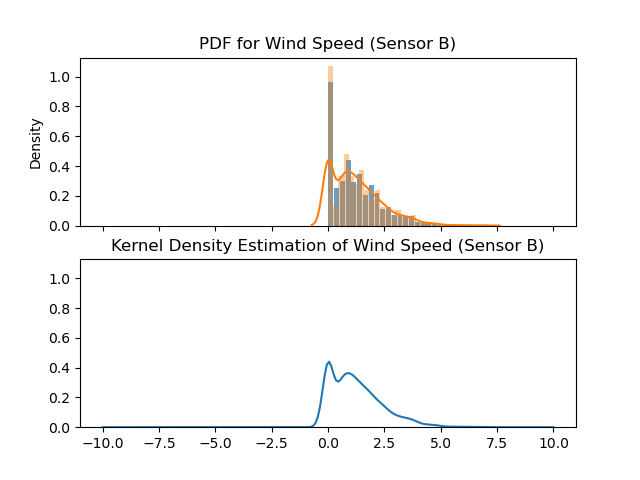
\includegraphics[width=0.7\textwidth]{PDF for Wind Speed (Sensor B).png}
	\caption{PDF for Wind Speed (Sensor B)\cite{Maiullari2020}}
  \end{figure}
  \begin{figure}[H] 
	\centering
	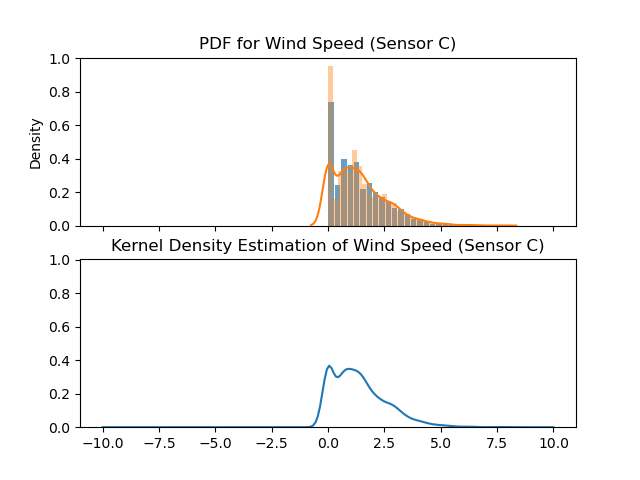
\includegraphics[width=0.7\textwidth]{PDF for Wind Speed (Sensor C).png}
	\caption{PDF for Wind Speed (Sensor C)\cite{Maiullari2020}}
  \end{figure}
  \begin{figure}[H] 
	\centering
	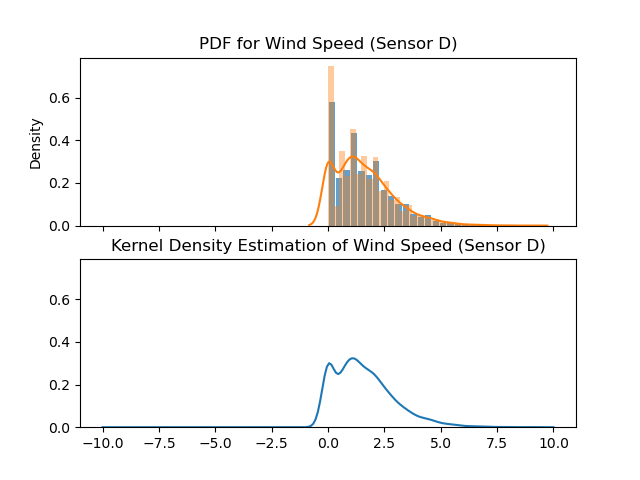
\includegraphics[width=0.7\textwidth]{PDF for Wind Speed (Sensor D).png}
	\caption{PDF for Wind Speed (Sensor D)\cite{Maiullari2020}}
  \end{figure}
  \begin{figure}[H] 
	\centering
	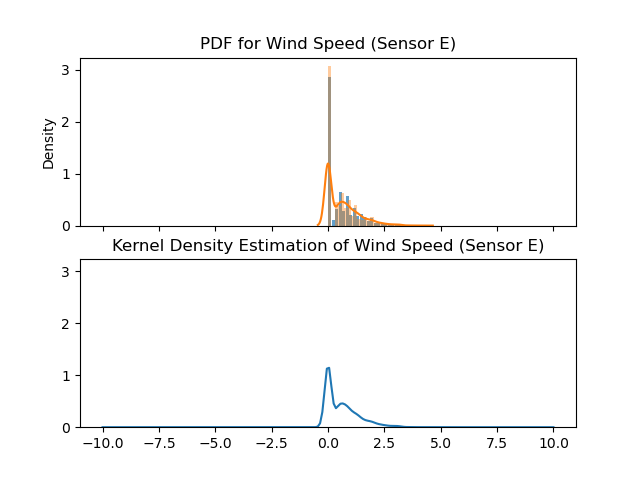
\includegraphics[width=0.7\textwidth]{PDF for Wind Speed (Sensor E).png}
	\caption{PDF for Wind Speed (Sensor E)\cite{Maiullari2020}}
  \end{figure}
\pagebreak
\section{A3}
 \subsection{A3.1}
  \begin{figure}[H] 
 	\centering
 	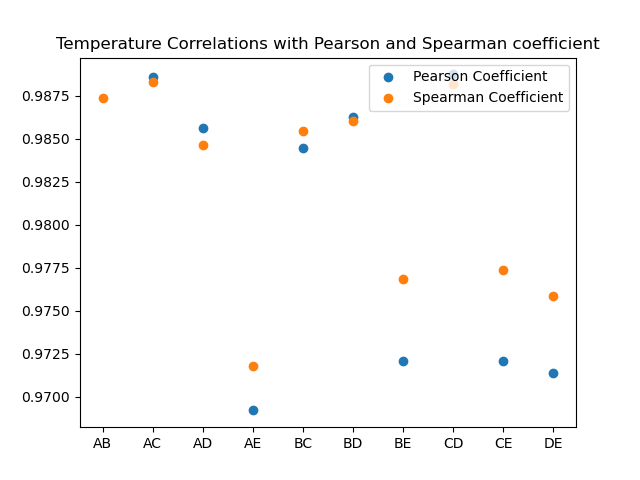
\includegraphics[width=0.7\textwidth]{Temperature Correlations with P and Sp coeff.png}
 	\caption{Temperature Correlations with P and Sp coeff\cite{Maiullari2020}}
  \end{figure}
  \begin{figure}[H] 
 	\centering
 	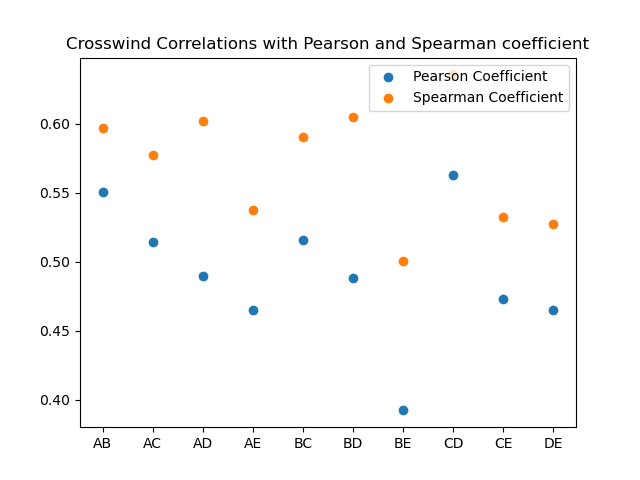
\includegraphics[width=0.7\textwidth]{Crosswind Correlations with P and Sp coeff.png}
 	\caption{Crosswind Correlations with P and Sp coeff\cite{Maiullari2020}}
  \end{figure}
  \begin{figure}[H] 
 	\centering
 	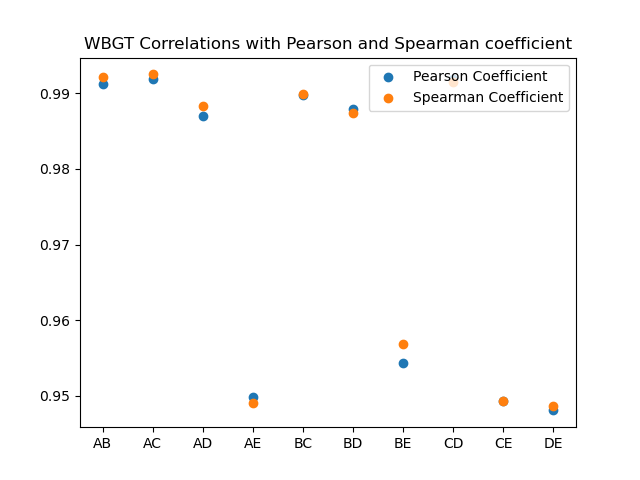
\includegraphics[width=0.7\textwidth]{WBGT Correlations with P and Sp coeff.png}
 	\caption{WBGT Correlations with P and Sp coeff\cite{Maiullari2020}}
  \end{figure}
 \subsection{A3.2}
 What we could say about the sensors correlations is that mostly they have high correlation since most of them are really near to 1 as about the Temperature and WBGT which means the temperature values they have measure are pretty similar to each other and that could happen because the sensors are in the same area and not really far from each other. About Crosswind since the correlation is around 0.5 means obviously that its not so high like the temperature values and that could mean either they are not so near or the winds in that area are a lot and gives us these results. The results could be seen the Table 1 and to Figures 15,16,17 above.
 \subsection{A3.3}
 With a good look in the correlations of the sensors we could say that from the temperatures the A-B and A-C sensors appear to have the highest correlation but at the same time they have low correlation as about the Crosswind. That is something which happens with all the sensors pairs actually. In that case it would unsafe to hypothesize which is the correct place for the sensors because all of them are quite near and so that means the temperature should be similar and therefore the correlation high. As about the crosswind correlation it could easily be low because the sensors are in an semi urban area and the crosswind could affect the correlation. In that case no specific hypothesize could be done.
   \begin{table}[]
 	\centering
 	\begin{tabular}{llll}
 		\hline
 		\multicolumn{1}{|l|}{Sensors Relationships} & \multicolumn{1}{l|}{Variables}   & \multicolumn{1}{l|}{Pearson Coefficient} & \multicolumn{1}{l|}{Spearman Coefficient} \\ \hline
 		\multicolumn{1}{|c|}{}                      & \multicolumn{1}{l|}{Temperature} & \multicolumn{1}{l|}{0.98810313}          & \multicolumn{1}{l|}{0.987378955}          \\ \hline
 		\multicolumn{1}{|c|}{AB}                    & \multicolumn{1}{l|}{Crosswind}   & \multicolumn{1}{l|}{0.550352585}         & \multicolumn{1}{l|}{0.596982562}          \\ \hline
 		\multicolumn{1}{|l|}{}                      & \multicolumn{1}{l|}{WBGT}        & \multicolumn{1}{l|}{0.991259553}         & \multicolumn{1}{l|}{0.992132436}          \\ \hline
 		& Temperature                      & 0.988608719                              & 0.988292007                               \\
 		\multicolumn{1}{c}{AC}                      & Crosswind                        & 0.51405088                               & 0.577228891                               \\
 		& WBGT                             & 0.99189585                               & 0.992472018                               \\ \hline
 		\multicolumn{1}{|l|}{}                      & \multicolumn{1}{l|}{Temperature} & \multicolumn{1}{l|}{0.985613462}         & \multicolumn{1}{l|}{0.984627239}          \\ \hline
 		\multicolumn{1}{|c|}{AD}                    & \multicolumn{1}{l|}{Crosswind}   & \multicolumn{1}{l|}{0.489895013}         & \multicolumn{1}{l|}{0.601889059}          \\ \hline
 		\multicolumn{1}{|l|}{}                      & \multicolumn{1}{l|}{WBGT}        & \multicolumn{1}{l|}{0.987013949}         & \multicolumn{1}{l|}{0.988291923}          \\ \hline
 		& Temperature                      & 0.969204792                              & 0.9717698                                 \\
 		\multicolumn{1}{c}{AD}                      & Crosswind                        & 0.465124685                              & 0.537844665                               \\
 		& WBGT                             & 0.949828692                              & 0.949127535                               \\ \hline
 		\multicolumn{1}{|l|}{}                      & \multicolumn{1}{l|}{Temperature} & \multicolumn{1}{l|}{0.98448517}          & \multicolumn{1}{l|}{0.985440109}          \\ \hline
 		\multicolumn{1}{|c|}{BC}                    & \multicolumn{1}{l|}{Crosswind}   & \multicolumn{1}{l|}{0.516102417}         & \multicolumn{1}{l|}{0.590683619}          \\ \hline
 		\multicolumn{1}{|l|}{}                      & \multicolumn{1}{l|}{WBGT}        & \multicolumn{1}{l|}{0.989729694}         & \multicolumn{1}{l|}{0.989863576}          \\ \hline
 		& Temperature                      & 0.986265403                              & 0.986048723                               \\
 		\multicolumn{1}{c}{BD}                      & Crosswind                        & 0.488029338                              & 0.604818597                               \\
 		& WBGT                             & 0.987864209                              & 0.987374811                               \\ \hline
 		\multicolumn{1}{|l|}{}                      & \multicolumn{1}{l|}{Temperature} & \multicolumn{1}{l|}{0.972089738}         & \multicolumn{1}{l|}{0.976859613}          \\ \hline
 		\multicolumn{1}{|c|}{BE}                    & \multicolumn{1}{l|}{Crosswind}   & \multicolumn{1}{l|}{0.39214871}          & \multicolumn{1}{l|}{0.500281016}          \\ \hline
 		\multicolumn{1}{|l|}{}                      & \multicolumn{1}{l|}{WBGT}        & \multicolumn{1}{l|}{0.95440893}          & \multicolumn{1}{l|}{0.956900474}          \\ \hline
 		& Temperature                      & 0.988742872                              & 0.988185589                               \\
 		\multicolumn{1}{c}{CD}                      & Crosswind                        & 0.562888199                              & 0.635906168                               \\
 		& WBGT                             & 0.991820559                              & 0.991421934                               \\ \hline
 		\multicolumn{1}{|l|}{}                      & \multicolumn{1}{l|}{Temperature} & \multicolumn{1}{l|}{0.972097215}         & \multicolumn{1}{l|}{0.977342412}          \\ \hline
 		\multicolumn{1}{|c|}{CE}                    & \multicolumn{1}{l|}{Crosswind}   & \multicolumn{1}{l|}{0.473233228}         & \multicolumn{1}{l|}{0.532232093}          \\ \hline
 		\multicolumn{1}{|l|}{}                      & \multicolumn{1}{l|}{WBGT}        & \multicolumn{1}{l|}{0.949269532}         & \multicolumn{1}{l|}{0.949345587}          \\ \hline
 		& Temperature                      & 0.971365706                              & 0.975848255                               \\
 		\multicolumn{1}{c}{DE}                      & Crosswind                        & 0.465192078                              & 0.527325327                               \\
 		& WBGT                             & 0.948090212                              & 0.94870202                               
 	\end{tabular}
 	\caption{Correlations between all the sensors for the variables: Temperature, Wet Bulb Globe Temperature (WBGT), Crosswind Speed\cite{Maiullari2020}}
 \end{table}
  \begin{figure}[H] 
	\centering
	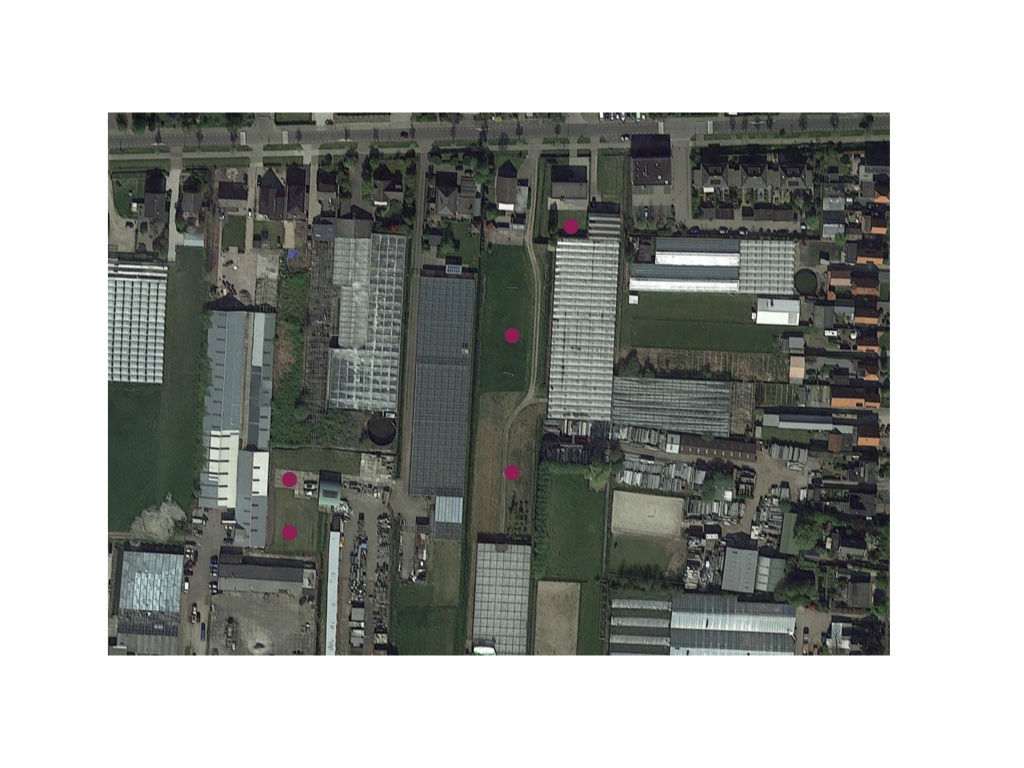
\includegraphics[width=0.9\textwidth]{Sensors Location.png}
	\caption{Sensors Location}
  \end{figure}
\section{A4}
 \subsection{A4.1,2}
   \begin{figure}[H] 
 	\centering
 	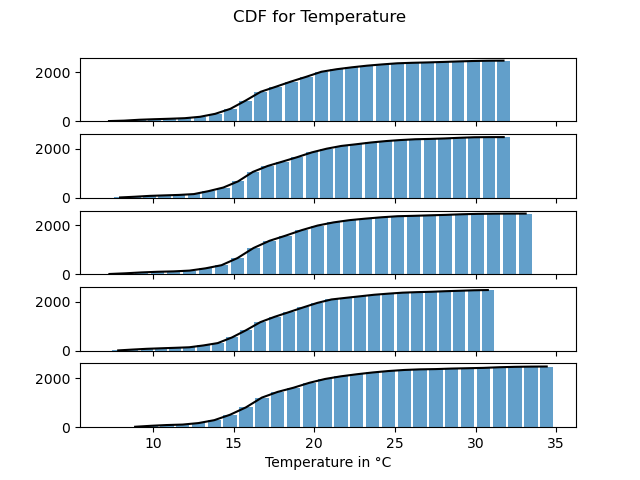
\includegraphics[width=0.7\textwidth]{CDF for Temperature.png}
 	\caption{CDF for Temperature\cite{Maiullari2020}}
   \end{figure}
   \begin{figure}[H] 
	\centering
	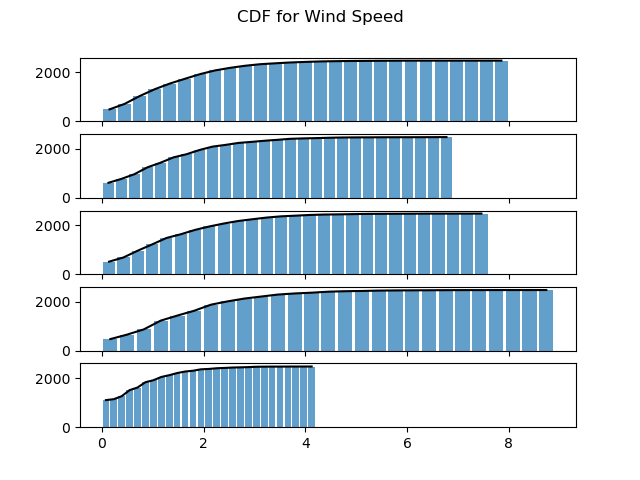
\includegraphics[width=0.7\textwidth]{CDF for Wind Speed.png}
    \caption{CDF for Wind Speed\cite{Maiullari2020}}
   \end{figure}
 \subsection{A4.3}
 So in the Table 3 below is visible the p-values from the requested sensors. We can conclude that most of them as about the temperature values (3 out of 4) are way above the 0.05 so that can strengthen the Hypothesis. And totally the opposite is happening with the Wind speed where we could say for the ED, DC, CB that we totally reject the hypothesis and that means the time series are different. Concluding what could be said is that obviously the p-value is not enough to reach a clear conclusion but probably none of the time series are completely the same so the Hypothesis could be rejected.
 \begin{table}[]
	\centering
	\begin{tabular}{|l|r|r|r|c|}
		\hline
		\multirow{2}{*}{Variables}                         & \multicolumn{3}{c|}{Confidence Intervals}                                    & \multicolumn{1}{l|}{\multirow{2}{*}{Sensors}} \\ \cline{2-4}
		& \multicolumn{1}{l|}{m-h} & \multicolumn{1}{l|}{m} & \multicolumn{1}{l|}{m+h} & \multicolumn{1}{l|}{}                         \\ \hline
		\multicolumn{1}{|c|}{\multirow{5}{*}{Temperature}} & 17.8121                  & 17.9691                & 18.1261                  & A                                             \\ \cline{2-5} 
		\multicolumn{1}{|c|}{}                             & 17.9047                  & 18.0654                & 18.2261                  & B                                             \\ \cline{2-5} 
		\multicolumn{1}{|c|}{}                             & 17.7549                  & 17.9131                & 18.0713                  & C                                             \\ \cline{2-5} 
		\multicolumn{1}{|c|}{}                             & 17.8381                  & 17.9964                & 18.1546                  & D                                             \\ \cline{2-5} 
		\multicolumn{1}{|c|}{}                             & 18.1819                  & 18.3539                & 18.5259                  & E                                             \\ \hline
		\multirow{5}{*}{Wind Speed}                        & 1.2462                   & 1.2903                 & 1.3344                   & A                                             \\ \cline{2-5} 
		& 1.1972                   & 1.2421                 & 1.2871                   & B                                             \\ \cline{2-5} 
		& 1.3243                   & 1.3715                 & 1.4186                   & C                                             \\ \cline{2-5} 
		& 1.5297                   & 1.5817                 & 1.6337                   & D                                             \\ \cline{2-5} 
		& 0.5681                   & 0.5962                 & 0.6244                   & E                                             \\ \hline
	\end{tabular}
	\caption{95/100 confidence intervals for variables Temperature and Wind Speed for all the sensors \cite{Maiullari2020}}
 \end{table}
 \begin{table}[]
	\centering
	\begin{tabular}{|c|r|r|c|}
		\hline
		\multicolumn{1}{|l|}{Sensors} & \multicolumn{1}{l|}{Student Test} & \multicolumn{1}{l|}{p value} & \multicolumn{1}{l|}{Variables} \\ \hline
		ED                            & 3.00023                           & 0.00271                      & \multirow{4}{*}{Temperature}   \\ \cline{1-3}
		DC                            & 0.72939                           & 0.46580                      &                                \\ \cline{1-3}
		CB                            & -1.32423                          & 0.18549                      &                                \\ \cline{1-3}
		BA                            & 0.84084                           & 0.40048                      &                                \\ \hline
		ED                            & -32.67317                         & 0.00000                      & \multirow{4}{*}{Wind Speed}    \\ \cline{1-3}
		DC                            & 5.87115                           & 0.00000                      &                                \\ \cline{1-3}
		CB                            & 3.89266                           & 0.00010                      &                                \\ \cline{1-3}
		BA                            & -1.50061                          & 0.13352                      &                                \\ \hline
	\end{tabular}
	\caption{Student Test and p-values}
 \end{table}
\pagebreak
\section{Bonus Question}
In this question it is asked to identify the hottest and coolest day of the measurement time series provided. In order to do that a python function created named (averagetemperature) which takes the data and calculates the maximum and minimum average temperatures in order to find which day is the hottest and coolest during the days that the data was acquired. In order to do that the function creates a table and sort it from the biggest to smaller value which in our case mean highest and coolest temperature. In that way we are able to find out the hottest and coolest days. From what the Table 4 above show us, the hottest day for the 4 out of 5 sensors was the 26th of June 2020 and the coolest the 10th of the same month. Finally only the E sensor had different days as the results show us.
\begin{table}[]
\centering
\begin{tabular}{|c|c|r|c|}
		\hline
		Sensors            & Hot/Cold & \multicolumn{1}{c|}{\begin{tabular}[c]{@{}c@{}}Temperature \\ \\ (Celsius)\end{tabular}} & Date      \\ \hline
		\multirow{2}{*}{A} & Hottest  & 25.1833                                                                                  & 6/26/2020 \\ \cline{2-4} 
		& Coolest  & 14.1556                                                                                  & 6/10/2020 \\ \hline
		\multirow{2}{*}{B} & Hottest  & 24.9292                                                                                  & 6/26/2020 \\ \cline{2-4} 
		& Coolest  & 14.3278                                                                                  & 6/10/2020 \\ \hline
		\multirow{2}{*}{C} & Hottest  & 24.8722                                                                                  & 6/26/2020 \\ \cline{2-4} 
		& Coolest  & 14.2667                                                                                  & 6/10/2020 \\ \hline
		\multirow{2}{*}{D} & Hottest  & 24.8750                                                                                  & 6/26/2020 \\ \cline{2-4} 
		& Coolest  & 14.3708                                                                                  & 6/10/2020 \\ \hline
		\multirow{2}{*}{E} & Hottest  & 25.9111                                                                                  & 6/25/2020 \\ \cline{2-4} 
		& Coolest  & 14.4903                                                                                  & 7/8/2020  \\ \hline
\end{tabular}
\caption{Highest and Lowest Temperature for every Sensor}
\end{table}
\pagebreak
\bibliographystyle{plain}

\bibliography{bibliography}
\end{document}
